\documentclass[conference]{IEEEtran}
\usepackage{graphicx}
\graphicspath{{fig/}}
\usepackage{balance}
\usepackage{amsmath, amssymb, amsbsy, pifont}
\usepackage{algorithm, algpseudocode}
\newtheorem{theorem}{Theorem}
\newtheorem{lemma}{Lemma}[theorem]
\newtheorem{definition}{Definition}
\usepackage{hyperref}
\usepackage{multirow}

\title{AcBF: A Revocable Blockchain-based Identity Management Enabling Low-Latency Authentication}
\author{Jianan Hong, Jia Cheng, Yuqing Li, Jiayue Zhou, and Yue Wu}
\begin{document}
\maketitle

\begin{abstract}
	Blockchain-based identity brings in great evolution due to its decentralized deployment, transparent and tamper-free ledger. Specification groups of B5G/6G are exploring approaches to integrate the technology to future network systems, e.g., Internet of Things, vehicular network, industrial communications. Note that devices in these systems are storage constrained with instable channels, thus requires lightweight node deployment. The security problem comes: revoked identity can forge a legitimate authentication, since the lightweight verifier does not maintain the revocation transactions. 
	This paper hence proposes AcBF, a novel revocable identity management scheme. Especially, it enables extremely low authentication latency by allowing the lightweight node to query the certificate's status locally. To realize this feature trustly, we first design a revocation transaction based on accumulator-assisted Bloom filter to minimize the storage of certificate status structure. Secondly, we further construct the blockchain protocol, with which, no revocation event will slip on any lightweight ledger, even in an insecure or instable communication environment.  
	In addition, different from other no-CRL revocation mechanisms, AcBF brings much smaller impact on valid user to execute the revocation. %, and with quite a small probability.
	Security and performance analysis
	shows that AcBF has strong security and advantageous efficiency on both lightweight verifiers and certificate owners, thus suits identity management systems with low-latency constraints.
\end{abstract}
\begin{IEEEkeywords}
    Blockchain identity, revocation-aware authentication, lightweight node, low latency
\end{IEEEkeywords}

\section{Introduction}
Blockchain is an attractive technology for distributed identity management \cite{9075663} due to its security features, such as append-only and non-tempering storage, decentralized consensus, and reliable trust establishment. Compared with traditional identity system, such as PKI (public key infrastructure) \cite{pki}, the character of blockchain-based method suits better in current and future network systems, due to its ability to faithfully organize the trust for large amount of entities \cite{chenCertchainPublicEfficient2018a,yang2018blockchain}, particularly the trust relationship between CAs (certificate authorities). 
Therefore, the idea of blockchain-based identity can develop security for various network scenarios, including Internet of Thing (IoT) \cite{zhangBPAFBlockchainEnabledReliable2022a, cui2022efficient}, Internet of Vehicles (IoV)  \cite{8010820,singh2018branch}, where decentralized trust is critically required. 

Despite the decentralized trust organization introduced by blockchain, it also brings in many practical problems due to its certificate status query method. For blockchain-based identity, a certificate's status (e.g., registered, illegal, or revoked) should be queried from the ledger of blockchain, which is maintained by multiple blockchain nodes. That is the cause of problems or security threats for communication resource-constrained scenarios. Firstly, the transaction query requires several round trip time (RTT) between IoT devices (or vehicle) and at least one blockchain node, which costs unbearable delay for latency-strict cases, e.g., safety notification message of IoV; what is worse, the highly dynamic topology of these network system makes the routing of query response complex. Secondly, it is dangerous to  query certificate's status from only one node, which leads to the security bottleneck problem; and it makes the first problem even worse to refer to more blockchain nodes. A worse threat is that some network attack will isolate the device from legal blockchain nodes at the very time when the device needs to check a certificate. 
It is intuitive but infeasible to let every device keep up with the whole ledger of blockchain, since the distributed devices are lightweight nodes for resources, especially storage. 

This paper proposes a blockchain-based identity management scheme by deploying lightweight blockchain nodes. Rather than stores the whole data, a lightweight node only stores the block header information of each block, thus help the storage-constrained devices to check transaction status locally, with the method of \textit{simplified payment verification} (SPV). As a result, the validity check of identity is completed with extremely low latency, regardless of the communication quality or network attack. 

The property of lightweight node has attracted many researchers to deploy blockchain in IoT, industrial environments, etc.. However, we should take more issues into account, before utilizing it to manage users' and devices' identities. The core problem is revocation! Let us take the following instance: a user's $U$ identity is registered in block $i$, and is later revoked in block $j$. If $U$ wants to authenticate its identity to a lightweight node, it can easily succeed in this forge: as $U$'s certificate still has a valid SPV method for block $i$, and the lightweight node is not informed of the revocation based on the stored block headers, unless $U$ consciously hands it up. Although some blockchain-based identity management schemes have proposed well designed revocation method \cite{luoScalaCertScalabilityOrientedPKI2022a,  wang2020blockchain,jiaRedactableBlockchainDecentralized2022,chenCertchainPublicEfficient2018a}, they no longer work in our system, as they require the verifier to master the whole blockchain data. 

The work presented in this paper aims at proposing a trusted blockchain-based identity management scheme, whose authentication method well resists the revoked users' forging. The proposed work uses a short Bloom Filter to record the revoked certificates; and additionally leverages a pairing-based accumulator to achieve a precise certificate validity check, even with quite small storage. Different from related work, in order to tolerate the case when the forger controls the communication channel, we construst a new certificate management scheme (AcBF). In AcBF, with our designed revocation transaction and small-volume header structure, the lightweight verifier can be aware of the revocation events with only the received header, thus achieves trust local query to improve the efficiency and reliability. 

In summary, this paper makes the following contributions:
\begin{enumerate}
	\item We propose a lightweight on-chain certificate management, where the authentication phase costs negligible overhead to validate the status of the certificate. Specially, the CRL is composed by designed accumulator-assisted Bloom filter (which is AcBF named from), thus the filter length can be drastically shortened without the problem of false detection. 
	\item To the best of our knowledge, we are the first to enable low-latency and trusted authentication enabled by blockchain technology, which makes the lightweight node be aware of revocation event according to block header. As a result, the identity status can be queried locally by the resource-constrained verifiers.
	\item We implement AcBF in our tested environment, and evaluate its performance in terms of computation and storage overhead in various procedures. Results show that AcBF informs every revocation to lightweight node, even in untrust network environment, and the overhead is extremely small on both certificate owners and verifiers, thus quite suit scenarios like IoT and IoV.
\end{enumerate}

The rest of this paper is organized as follows. We will
introduce necessary preliminaries in Section \ref{sec:preliminary}, and in Section \ref{sec:model} we present the system model, followed with the security requirements of AcBF. Detailed Construction is presented in Section \ref{sec:construction}. Then formal security proof and experimental result analysis are shown in Section \ref{sec:security} and \ref{sec:efficiency}, respectively. Section \ref{section:related} briefly discusses the related work. Finally, in Section \ref{sec:conclusion}, we conclude this paper. 


\section{Preliminaries}\label{sec:preliminary}

\subsection{Bilinear Pairing}
Let $\mathbb{G}_1$, $\mathbb{G}_2$ and $\mathbb{G}_T$ be 3 groups of prime order $p$. A pairing map $e:\mathbb{G}_1\times \mathbb{G}_2\rightarrow\mathbb{G}_T$ satisfies:
\begin{itemize}
	\item \textit{Bilinearity:} for all $(x,y, g_1, g_2) \in \mathbb{Z}_p^2\times \mathbb{G}_1\times \mathbb{G}_2$, $e(g_1^x, g_2^y) = e(g_1, g_2)^{xy}$;
	\item \textit{Non-degeneracy:} if $g_1, g_2$ are generators of $\mathbb{G}_1$ and $\mathbb{G}_2$, respectively, $e(g_1, g_2)$ generates $\mathbb{G}_T$;
	\item \textit{Efficiency:} It is efficient to compute $e(u,v)$ for all $(u, v) \in \mathbb{G}_1\times \mathbb{G}_2$.
\end{itemize}

According to the relationship of $\mathbb{G}_1$ and $\mathbb{G}_2$, there are three types of pairings \cite{GALBRAITH20083113}. 
In Type 1, $\mathbb{G}_1 = \mathbb{G}_2$; In Type 2, $\mathbb{G}_1 \neq \mathbb{G}_2$, but there is a unidirectional homomorphism $\phi:\mathbb{G}_2 \rightarrow \mathbb{G}_1$; An in Type 3, no PPT homomorphism algorithm exists between the two groups.
Overall speaking, Type 3 pairings are more secure and efficient to map, which is used in this paper.

Consider the $q$-Strong Diffie-Hellman Problem ($q$-SDH) \cite{Boneh2004} as follows: given a tuple $(g_1, g_2, g_2^{\gamma}, g_2^{(\gamma^2)}, \dots, g_2^{(\gamma^q)})$ as input, where $g_1\in\mathbb{G}_1$, $g_2\in\mathbb{G}_2$, and $\gamma\in \mathbb{Z}_p$, outputs a pair $(g_1^{1/(\gamma + x)}, x)$ where $x \in \mathbb{Z}_p$. We say that an algorithm $\mathcal{A}$ has advantage $\epsilon$ in solving $q$-SDH if it has probability $\epsilon$ to return the valid pair.

\begin{definition}[$q$-SDH Assumption]
	No PPT algorithm $\mathcal{A}$ can has a non-negligible advantage $\epsilon$ for $q$-SDH problem.
\end{definition}


\subsection{Bloom Filter}\label{section:bf}
Bloom filter (or BF for short) is a space-efficient data structure to record a set, in order to support membership queries \cite{Bloom1970, broder2004network}.
BF is an array of $m$ boolean bits, whose initial status is all zeros (denoted as $0^m$). Another parameter $k$ is the number of independent hashes, each of which maps a member to a random bit of BF. The follows describe the functions of BF, which will be used in the later context.

\begin{itemize}
    \item $BF.Add(x)$: To add an element $x$ to BF, it respectively hashes $x$ with the $k$ hashes of BF, and sets each of the mapped bit to 1.
	\item $BF.Check(x)$: To query if $x$ has been added, it uses the $k$ hashes to map $x$ to a set of bits. If any of them is 0, it returns False; otherwise, it returns True. 
\end{itemize}

Especially, the $BF.Check()$ gives a False result with no doubt; whereas the True result has the potential to happen when the tested element has not been added, which means a false positive situation. 

\subsection{Merkle Tree and Simplified Payment Verification (SPV)}
\label{section:merkle}
Merkle hash tree \cite{merkle1987digital} is essentially a binary tree where the leaf node is labeled a hash of a data block, and the non-leaf node is labeled with the hash of its child nodes. Such structure allows efficient verification of any large data. As shown in Fig. \ref{fig:mht}, $cert_A$ is labelled with the 2nd leaf of MHT, whose path is ``01'' (0 for left child and 1 for the right).

Simplified payment Verification (SPV) is a method to check if one data block is in a MHT, when the verifier only knows the root node. To realize the verification, SPV requires the prover side to offer necessary auxiliary information to the verifier, which means the values of \textbf{all sibling nodes from the hash of proved data block to the root}.
Return to Fig. \ref{fig:mht}, the auxiliary information of $cert_A$ is as: $AUX_A = (h_{00}, h_{1})$. Since each one obtaining tuple $(R, cert_A, AUX_A)$ can check if:
\begin{align}\label{eq:aux}
R \overset{?}{=} h(h(h_{00}, h(cert_A)), h_1)
\end{align}
%where $h()$ is any selected secure hash function.

\begin{figure}[t]
	\centering
	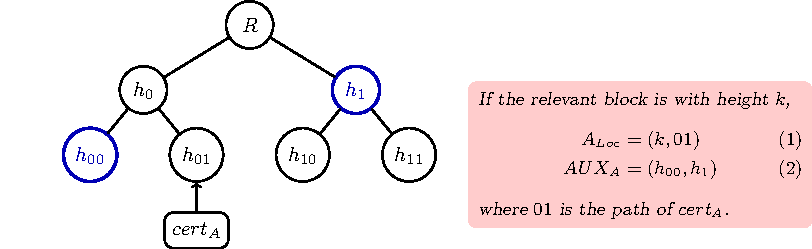
\includegraphics[width=8.5cm]{mht}
	\caption{Instance of merkle hash tree (MHT) with necessary definitions}\label{fig:mht}
\end{figure}

\section{System and Security Model} \label{sec:model}
As shown in Fig. \ref{fig:model}, the proposed scheme works in a communication system with the following 3 kinds of entities: multiple CAs, lightweight nodes and a set of blockchain full nodes. The follows describe each of the entities. 


\begin{figure}[t]
	\centering
	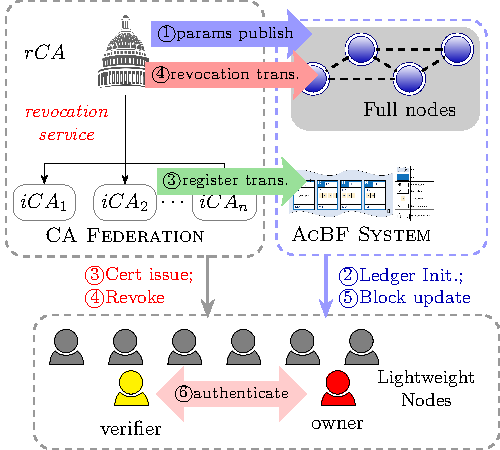
\includegraphics[width=7.5cm]{model}
	\caption{Blockchain-based Identity System Architecture}\label{fig:model}
\end{figure}
\subsection{Entity Description}
\subsubsection{Certificate Authorities}
 The CAs play the similar role as those in traditional PKI systems, which are responsible for issuing and revoking certificates for other entities. AcBF sepereates multiple CAs into two categories: one revocation CA (rCA) for certificate revocation, and muliptle issuer CAs (iCA) for issuing affairs. 
 
 The rCA should be responsible for parameter determination (as \textcircled{1} in Fig. \ref{fig:model}), and revoke on-chain certificates by \textcircled{4}submitting revocation transactions. Different from PKI, the iCAs are not fully trusted, they issue on-chain certificates to other entities by \textcircled{3}submitting registration transactions. 

It should be mentioned that, it is easy to fully decentralize AcBF by realizing a threshold revocation among muliple rCAs. There are exiting cryptographic solutions such as \cite{Gennaro2019FullyDG} to be leveraged. 
For the clarity of introduction, this paper just uses a one-rCA model. 

\subsubsection{Full Nodes}
They are blockchain nodes storing all blocks including transactions, and taking part in every-round consensus. Our scheme does not depend on a specific consensus method. The full nodes provide service to other entities: they gather transactions from CAs to generate blocks, \textcircled{5} broadcast latest block header to lightweight nodes, and \textcircled{2} help lightweight node to initiate local ledger,  when the lightweight nodes newly enters the system just then. 

\subsubsection{Lightweight Nodes}
They are resource constrained devices from the perspective of storage and bandwidth. Thus they only stores block header for transaction validation based on SPV method. 
To achieve the SPV, the lightweight node should keep up with the blockchain status by receiving newly generated blocks, as well as the revcation events from at least one reachable full nodes. 

The lightweight nodes will communicate with each other, thus should \textcircled{6} authenticate and convince the opponent that its identity is valid. On this aspect, each lightweight node play two roles: it is a verifier based on its lightweight leger; and also a certificate owner, that should maintain its authentiation parameters, including secret key and auxiliary information.

\subsection{Security Assumption}
In our system, the rCA, as a core entity, is totally trusted. It securely preserves the security of secret keys and honestly generates the revocation transactions. The iCAs are not strictly honest; whereas, any entity can determine the certificate credibility according to the trust level of relevant iCA. Luckily, the blockchain does well in constructing the trust. 

Any single blockchain full node is not honest, it may try responding spoofing transaction or hiding revocation event if it can benefit. However, the overall blockchain system is assumed safe and live based on the consensus mechanism; it is hard to send non-consensused block header due to the assumption of selected consensus mechanism. For instance, in PoW, malicious full nodes cannot succeed in puzzle solving game, thus leads to its shorter fork.

The lightweight nodes cannot be trusted, they try to forge a valid certificate status, even if it has been revoked. In addition, malicious nodes will even forge a full node to broadcast false header to others and control the links. As a verifier, we assume that they will try their best to update their local ledger to the correct version. 

This paper further assumes the communication links of lightweight node: 1) during long-lifetime interaction, the link is instable and insecure; 2) in its initialization phase, it has adequate resource to update its local ledger to the latest and correct version, including other variables, e.g., Bloom filter and accumulator.

\subsection{Design Goals}
Based on the security assumptions, AcBF should achieve the following properties as an efficient and secure scheme:  
\begin{itemize}
	\item \textit{Revocation-detectable authentiation.} Only user's with valid and non-revoked certificate can authenticate successfully, faced with lightweight node.
	\item \textit{Lightweight node-aware revocation.} No reocation event should slip on a lightweight node, even in an untrusted environment. 
	\item \textit{Low-latency authentiation.} Latency should be strictely restricted regardless of any situation. 
	\item \textit{Slight impact.} The above properties should be achieved without bringing much burden to honest entities, e.g, rCA and lightweight nodes.
\end{itemize}
\section{Construction}\label{sec:construction}
\subsection{Revocation-Aware Block Format}
\label{sec:format}
The block structure in this paper is basically similar to that of Bitcoin, except for the consideration of lightweight node awareness. Firstly, the storage cost of block header should be as short as possible with efficient query and sacrificing no security feature; Secondly, the block header alone can prompt every certificate revocation clearly. 

Taking into account the two issues, we redesign the 1) fields of block header, and 2) the tree structure of transactions. The header is a fixed length data, such that an unstructured storage can support fast addressing based on block height. The necessary fields are depicted in Table \ref{table:format}. Especially, as our later implementation uses 224-bit hash function and curves, the presented sizes of Previous hash and MHT (hash of merkle hash tree) are 28 bytes. The Flag field is a main difference for the second consideration: it is a boolean variable to notify whether revocation events occur in this round.

The consensus field depends on the used consensus method, e.g., it is a nonce for puzzle-like consensus method like PoW, or a digital signature for permission-based consensus.


\begin{table}[h] 
	\caption{Block Header Format}\label{table:format}
	\centering
	\begin{tabular}{c|c|l}
		\hline
		Field & Size & Description \\
		\hline
		Height & 4 bytes & An incremental integer to identify this block \\
		Previous Hash & 28 bytes & A hash of previous block \\
		Flag & 1 bit & Indication of revocation \\
		MHT & 28 bytes & Hash of all transactions in this block \\
		Consensus & \textit{variable} & Some method proving the validity of block\\
		\hline
	\end{tabular}
\end{table}

All registered certificates (regarded as transactions) are structured in merkle hash tree as Section \ref{section:merkle}, whose hash of root node is represented as $R_c$. There is also a slight difference for revocation awareness: if there is no revocation, $R_c$ is just the value of MHT; otherwise, MHT is assigned the hash of $R_a$ and the signature of revocation transaction in this block (denoted as $R_x$). For certificates registered in this block, their SPV data includes $R_x$ in such case.


\subsection{System Procedures}

\subsubsection{Initialization}
The rCA initiates the system by generating a bilinear tuple $PP=\{p, \mathbb{G}_1, \mathbb{G}_2, \mathbb{G}_T, g_1, g_2, e\}$ and a hash function $H:\{0, 1\}^* \rightarrow \mathbb{Z}_p$. It selects its master secret key $\gamma\in \mathbb{Z}_p$, accumulator value $\Delta\in_R \mathbb{G}_1$, 
and parameters of Bloom filter $(m, k)$ as Section \ref{section:bf}, based on the expected system scale as Section \ref{section:parameter}. It further generates an empty revocation list $\mathbb{R}_x$. The system parameters are published as 
$$ \bigl\{ PP, \Delta, Y = g_2^\gamma, (m, k), H \bigr\}$$

Blockchain full nodes are gathered by generating a genesis block $B_0$, whose header's format follows Table \ref{table:format}, with all-zeros fields, except the consensus. 

The iCAs are registered in the blockchain as Section \ref{section:register}. As a distributed system, iCA's certificates should be registered in self-sovereign manner, while our AcBF also supports rCA's issuing, by using key pair $(\gamma, Y)$ under any signature algorithm. Note that, iCA's certificate status is queried like other entities', hence the later content will not specifically describe the iCA's status check in authentication phase. 


Every lightweight node initiates its ledger by updating the block headers from selected full nodes, like other lightweight node-supported schemes. In addition, it updates the Bloom filter $BF$ and accumulator value $\Delta$. As the full nodes are not trusted, the $BF$ and $\Delta$ are checked from the blocks with revocation transactions as depicted in Section \ref{sec:revoke}.

\subsubsection{Certificate Register}\label{section:register}
From an arbitrary trusted iCA, each entity $U_i$ applies this phase to register an on-chain certificate $cert_i$. The certificate in AcBF is basically similar to that in X.509, except that AcBF does not need the globally unique sequence number. Instead, AcBF uses its unique location $i_{Loc} = (i_h, i_p)$ in blockchain to identify the certificate, where $i_h$ is denoted as the height of registered block, and $i_p$ is its path in MHT. Fig. \ref{fig:mht} gives an instance of a certificate's unique location. 

$U_i$ securely stores a secret key $sk_i$, whose relevant public key $pk_i$ is included in $cert_i$. The $U_i$ should wait for this certificate to be gathered with other transactions (including registration and revocation transactions). After the consensus and broadcast of the block as Section \ref{section:block_consensus}, this phase is completed with $U_i$ gets its $i_{Loc}$ and the auxiliary information of MHT $AUX_i$.


\subsubsection{Revocation} \label{sec:revoke}
This phase consists of 1) execution by rCA, and 2) reaction by other entities, especially the lightweight nodes. 

1) To execute revocation, rCA prepares a temporary revocation list $\mathbb{R}$ gathers revocation request from legal iCAs and certificate owners. After validation of each request (which is beyond the scope of this paper), rCA appends the location $i_{Loc}$ of the certificate to $\mathbb{R}$ until it invokes Algorithm \ref{alg:revokeCA} to generate revocation transaction. 


\begin{algorithm}[t]
\renewcommand{\algorithmicensure}{\textbf{Output:}}
	\caption{Revocation Procedure of rCA}\label{alg:revokeCA}
	\begin{algorithmic}[1]
		\Require $\mathbb{R}$, $\mathbb{R}_x$, $BF$ and $\Delta$ %\Comment{Set of user indexes to be revoked}
		\Ensure Revocation Transaction ($rx$)
		\State $L\gets \emptyset$
		%\State $\Delta_T \gets \Delta$
		\State $BF_{tmp} \gets 0^m$ \Comment{Empty Bloom filter}
		\ForAll{$x \in \mathbb{R}$}
		\If{$BF.Check(x)$} %\Comment{as Section \ref{section:bf}}
		\State $\Delta \gets Del(\Delta, x)$ \Comment{as Algorithm \ref{alg:accumulate}}
		\State append $(x, \Delta)$ to L
		\Else
		\State $BF_{tmp}.Add(x)$ %\Comment{as Section \ref{section:bf}}
		\EndIf
		\EndFor
		\State $BF \gets BF \lor BF_{tmp}$, $\mathbb{R}_x \gets \mathbb{R}_x \bigcup \mathbb{R} $
		
		\Return $rx \gets (L, \mathbb{R})$
	\end{algorithmic}
\end{algorithm}

Especially, AcBF proposes an efficient accumulator method based on \cite{accumulator}, including the following three functions:
\begin{itemize}
	\item \textit{Add} makes the input value $x_i$ as the member of accumulator, by outputting $W_i$ as its witness;
	\item \textit{Del} removes the member $x_i$ by updating the value $\Delta$;
	\item \textit{Update} helps the other members $x_i$ to update their witnesses with the input parameters.
\end{itemize}
The detailed execution of these functions are illustrated in Algorithm \ref{alg:accumulate}.
Then, rCA submits $rx$ along with the signature $R_x$ to the blockchain nodes, using its secret key $\gamma$.

\begin{algorithm}[t]
	\renewcommand{\algorithmicensure}{\textbf{Output:}}
	\caption{Accumulator}\label{alg:accumulate}
	\begin{algorithmic}[1]
		\Require $\gamma, \Delta, Y= g_2^\gamma$ %\Comment{Set of user indexes to be revoked}
		%\Ensure Revocation Transaction ($rx$)
		\Function{Add}{$\Delta, x_i$}
		
		\Return $W_i \gets \Delta ^{1/(x_i + \gamma)}$
		\EndFunction
		
		\Function{Del}{$\Delta, x_j$}
		
		\Return $\Delta \gets \Delta ^{1/(x_j + \gamma)}$
		\EndFunction
		\Function{Update}{($x_i, W_i), \Delta, x_j$} \Comment{$x_j$ is revoked}\label{fuction:update}
		
		\Return $W_i \gets (W_i/\Delta)^{1/(x_j - x_i)}$
		\EndFunction
	\end{algorithmic}
Note that, as $x_i$ in AcBF is a location, the real input uses $H(x_i)$ to replace $x_i$. 
\end{algorithm}

2) When a lightweight node $U_i$ invokes the revocation by the notification of Flag field as Section \ref{section:block_consensus}, it updates the maintained BF and $\Delta$ with the revocation transaction $rx$. Parse $rx$ as $(L, \mathbb{R})$ and executes Algorithm \ref{alg:revokeNode}.

Worth noting that, Line \ref{line:apply_accumulator} of this algorithm focuses on the case a legal user will be innocently checked as revoked one if only with Bloom filter. Whereas, AcBF uses the accumulator $\Delta$ to fix this problem. The rCA will be responsible for this request since it has the entire revocation list $\mathbb{R}_x$.

\begin{algorithm}[t]
	\renewcommand{\algorithmicensure}{\textbf{Output:}}
	\caption{Revocation Reaction by Lightweight Node $U_i$}\label{alg:revokeNode}
	\begin{algorithmic}[1]
		\Require $BF, i_{Loc}, L, \mathbb{R}, W_i$. \Comment{$W_i$ is input only if $i_{Loc}\in\Delta$}
		\Ensure $\Delta$
		\If{$L\neq\emptyset$}
		\State Update $\Delta$ as the last tuple of $L$
		\EndIf
		\ForAll{$x \in \mathbb{R}$}
		\State $BF.Add(x)$ 
		\EndFor
		\If{$W_i$ is input} 
		\ForAll{$(x_j, \Delta) \in L$}
		\State $W_i\gets Update((i_{Loc}, W_i), \Delta)$ \Comment{Line \ref{fuction:update} of Alg. \ref{alg:accumulate}}
		\EndFor
		\ElsIf{$BF.Check(i_{Loc})$}
		\State Invoke $Add(\Delta, i_{Loc})$ with rCA to get $W_i$ \label{line:apply_accumulator}
		
		\Return $W_i$ as $U_i$'s witness
		\EndIf
	\end{algorithmic}
\end{algorithm}

\subsubsection{Authentication}\label{section:authentication}
When $U_i$ needs to authenticate itself to a lightweight verifier $V$, it should sign a certain message or a challenge with its $sk_i$. This paper focuses on the issue that how $U_i$ convinces $V$ that the relevant $pk_i$ is associated with a valid on-chain certificate.

The certificate validation message includes the certificate $cert_i$, its registered location $i_{Loc}$ (including $i_h$ and $i_p$), the auxiliary information of MHT $AUX_i$. If $U_i$ has got $W_i$, the witness of accumulator, then $W_i$ should also be in the message. The entire message is as 
$$\sigma = \biggl(Sig(m; sk), cert_i, i_{Loc}, AUX_i, \mbox{\textit{optional }} W_i\biggr)$$

Upon the recept of $\sigma$, $V$ checks the follows:
\begin{itemize}
	\item \textit{Existence}: the tuple $(R, cert_i, AUX_i)$ as \eqref{eq:aux}, where $R$ is the MHT field of the $i_h$-th block.
	\item \textit{Non-revocation}: If $\sigma$ does not contain $W_i$, checks $$BF.Check(i_{Loc})\overset{?}{=} 0;$$ Else, checks 
	\begin{align} \label{eq:authenticate}
		e(W_i, g^{H(i_{Loc})}\cdot Y) \overset{?}{=} e(\Delta, g_2)
	\end{align}
	\item The signature is validated with public key in $cert_i$.
\end{itemize}
If the above is all passed, $V$ is convinced that $U_i$ is valid. Otherwise, the authentiation is failure. 


\subsubsection{Block Generate and Broadcast}\label{section:block_consensus}

The blockchain full nodes collect certificate register transactions from muliptle iCAs, and at most one revocation one $rx$ (with signgature $R_x$). According to the selected consensus mechanism, the nodes organize the transactions to MHT, according to Section \ref{sec:format}, as well as the block header encapsulation: the Flag field is set to ``1'' or ``0'', depending on whether this block contains an $rx$. Let the height of this newly generated block be $h_n$.

After this block is generated, other full nodes checks its validity including the follows:
\begin{itemize}
	\item \textit{Transactions:} All transactions are valid, especially, $R_x$ is the correct signature of $r_x$ with $Y$.
	\item \textit{Structure:} $h_n = h_c + 1$, where $h_c$ is the largest height of stored block; $rx$ exists if Flag is ``1''; and all hashes are valid, including the previous hash.
\end{itemize}

After consensus, the block header, as well as $r_x$ and $R_c$ (the MHT root of only certificate registration transaction) are transmitted to every lightweight node. 
Upon the recept of the header, each lightweight node checks as: 
\begin{enumerate}
	\item If Flag is ``1'' without $rx$, the lightweight node should request $rx$ as well as $R_c$. Otherwise, finishes the check.
	\item  Check $R_x$ is the signature of $r_x$ and $H(R_a, R_x) \overset{?}{=} R_c$, which is the value of MHT field of this block. 
\end{enumerate}

Whether full or lightweight nodes, if the Flag is ``1'', then invokes Algorithm \ref{alg:revokeNode} with the verified $rx$, to update local BF, accumulator value $\Delta$ and optionally its witness.
After that, the lightweight node removes $r_x$, $R_x$ and $R_a$.

\subsection{Parameter Determination for Bloom Filter} \label{section:parameter}

The length of Bloom Filter in this paper can be dramatically decreased compared with other schemes for certificate revocation. This section gives a theoretical derivation for the relevant parameter.

Let $n, \delta$ be the possible maximal number of registered and revoked users, respectively. The remaining factor is system effect of user revocation: when revocation is executed in one consensus round, the expected affected users should be limited to $\theta$, which can be measured as the member amount of Accumulator $\Delta$. The measurement is feasible as:
\begin{itemize}
    \item Larger member amount in $\Delta$ causes larger probability that a user to be revoked has already in $\Delta$ and more other members to update their witness.
    \item The probability that innocent users applies for accumulator member affects the increase rate of $\theta$. Thus, $\theta$ also implies the effect when revocation is executed just in Bloom filter.
\end{itemize}

Assume $m$ is the calculated hash length with $k$ hash functions in the Bloom filter. With $\delta$ users already be revoked, the probability can be measured as follows, that an legal user is erroneously claimed as a revoked one: 
\begin{align} 
    \Pr(1) \simeq (1 - e^{-k\delta/m})^k 
 \end{align}

The parameter $k$ can be individually optimized to minimize $\Pr(1)$ as $ k = \frac{m}{\delta}\ln 2$. Then, for $n$ valid users, the expected affected amount (limited to $\theta$) is 
\begin{align}\label{eq:bloomfilter}
    \theta = n \cdot (1 - e^{-k\delta/m})^{k} = 0.5^{\frac{m}{\delta}\ln 2}\cdot n
\end{align}
From \eqref{eq:bloomfilter}, the parameters of Bloom filter are determined as 
\begin{align}
m = & \frac{\ln \frac{n}{\theta} \cdot \delta}{(\ln 2)^2} \simeq 2.08\delta \cdot\ln \frac{n}{\theta}\\
k = & \lfloor \ln \frac{n}{\theta} / \ln 2 \rceil \simeq \lfloor 1.44 \ln \frac{n}{\theta} \rceil
\end{align}

%\subsection{Compatibility on Other Blockchains}
%We recommend to implement AcBF with designed block header structure as Table \ref{table:format}, but it is also compatible with traditional blockchain implementations. The main challenge is that Flags

\section{Security Analysis of AcBF}\label{sec:security}
\subsection{Sound Authentication and Reliable Revocation}
\begin{theorem}\label{theo:security}
	The AcBF identity management achieves sound and revocation-detectable user authentication for the lightweight-node verifier.
\end{theorem}

\begin{IEEEproof}
    A user without a registered certificate in public ledger (even without a revoked identity) will not forge an authentication due to the traditional certificate technique with trust SPV method. Thus, this proof mainly focuses on the revoked user. Formally, this theorem holds if a revoked user $\mathcal{A}$ wins the following challenges with negligible advantage.
    \begin{enumerate}
        \item With the knowledge of accumulator value $\Delta$, as well as any other user's accumulator pair from authentication message $(i_{Loc}, W_i)$, $\mathcal{A}$ tries to forge its witness.
        \item When $\mathcal{A}$ goes through a revocation based on member delete in $\Delta$, it tries to forge a new witness value for the updated $\Delta$.
        \item When $\mathcal{A}$ is revoked in block $j$, it tries to hide the revocation fact during the broadcast of block header.
    \end{enumerate}

    The first 2 challenges require a secure cryptographic accumulator, and a strong blockchain protocol is in need for the last challenge. Hence, the demonstration of Theorem \ref{theo:security} can be derived from the following 2 lemmas.
\end{IEEEproof}
\begin{lemma}
    If $q$-SDH assumption holds, the revocation method based on accumulator mechanism in Algorithm \ref{alg:accumulate} is sound against revoked identities.
\end{lemma}
\begin{IEEEproof}
	The accumulator algorithm was basically proved secure under $q$-SDH assumption in \cite{accumulator}, whereas, AcBF makes two modifications. Firstly, we remove the zero-knowledge proof (ZKP) to accelerate the authentication phase as \eqref{eq:authenticate}; Secondly, \textit{Add} function inserts an arbitrary member value without changing the accumulator public value $\Delta$. 
	
	In fact, non-ZKP authentication only helps the adversary $\mathcal{A}$ to get the member secret (or the unique location $i_{Loc}$ in AcBF) and its witness $W_i$, compared with standard algorithm. Whereas, the $i_{Loc}$ is no longer secret in AcBF, and $\mathcal{A}$ cannot learn the information of the secret key $sk_i$, which is relevant to the public key in the transaction recorded in $i_{Loc}$. Thus, as long as the consensus mechanism is safe (to ensure that every $i_{Loc}$ is unique between certificates), the additional information in \eqref{eq:authenticate} brings no advantage to adversaries. On the other hand, we analyze the advantage from cryptographic perspective. A tuple $(\Delta, x, W = \Delta^{1/(x + \gamma)})$ can be reduced to $(B=h^{x+\gamma}, x, h)$, which leaks no knowledge on $\gamma$.
	
	The second modification makes our accumulator be a stand $q$-SDH tuple: Given as system with a secret key $\gamma$, and public group elements $\Delta \in \mathbb{G}_1$, $(g_2, Y = g_2^\gamma)\in \mathbb{G}_2$. The hash of member value and its witness ($H(i_{Loc}), W_i$) is identical to the tuple $(x, \Delta^{1/(x+\gamma)})$. 

	The Member \textit{Del} and \textit{Update} function in Algorithm \ref{alg:accumulate} is also identical to key revocation in BBS signature \cite{Boneh2004}. A intuitive description about the revocation capability is that the revoked user $U_j$ should deal with the problem of zero denominator to update its witness, as $x_i=x_j$. Formal reduction from BBS signature to $q$-SDH assumption is given in \cite{Boneh2004}. As our modified accumulator can be reduced to BBS, it is sementically secure under $q$-SDH assumption. 
\end{IEEEproof}
\begin{lemma}
    If the consensus protocol of the used blockchain is safe, the lightweight node is aware of every revocation when its ledger has been updated to relevant status.
\end{lemma}

\begin{IEEEproof}
When a certificate is successfully revoked in a block (e.g., of height $i$), the Flag field of its header should be \textit{True}. As long as the consensus protocol has a strong safety property, the lightweight node $V$ will not accept the $i$-th block header with Flag field \textit{False}. 

With the above result, any revocation transaction should be sent to the $V$ with the signature $R_x$ and auxiliary information $R_c$, where $R_c$ is the root value of all certificate registration transactions in this block. No adversary can hide or modify even one revocation item in this scenario due to the unforgeable signature and hash strength, even by forging a full node or controling the downlink channel.
\end{IEEEproof}

\subsection{Lightweight Overhead}
AcBF achieves this property on two aspects. Firstly, a lightweight node requires no interaction with full nodes to validate any certificate's status, regardless of any cases, thus achieves extremely low-latency authentication. Secondly, it brings in slight impact on the system to maintain the reliable revcation.

On the first aspect, we use a short Bloom filter to record the revocation list, while uses accumulator to fix its false positive situation: a wronged user is a member of accumulator, thus achives fast authentication with an efficient member check as \eqref{eq:authenticate}. Without this method, when a user is checked as revoked, it requires the verifier to request relevant transaction from trusted full nodes to judge the real status. Furthermore, only wronged certificate needs additional check based on accumulator, the average latency is still similar to no-revocation method. 

On the second aspect, all entities cost negligible burden besides the basic block header update. 1) As a lightweight verifier, it only needs a short BF structure and an accumulator value to enable its validation ability. All revcation transactions should be erased after the verifier has update its BF and $\Delta$. 2) As an identity owner, it basically maintains the location and auxiliary information of its registered certificate. 3) Even as accumulator member, the \textit{Update} function only occurs when a user in accumulator is revoked, the probability is quite small. And compared with revocation based on smart contract or MHT, every user can update its witness with the public revocation transactions, thus costs no additional resources


\begin{table*}[t]
	\caption{Performance Comparison with Related Schemes}
	\label{table:compare}
	\centering
	\begin{tabular}{l | c |c| c | c |c c c | c}
		\hline\hline
		\multirow{2}*{Scheme} & Lightweight & \multirow{2}*{Revocable} & Revocatin & Additional &\multicolumn{3}{c|}{Revocation Impact on} & Issues faced with \\
		& node \textit{supp.} & & mechanism &method& Verifier  & Owner & System & lightweight node\\
		\hline
		CertChain \cite{chenCertchainPublicEfficient2018a} & \ding{55}& \checkmark & Bloom Filter & \textit{n/a} & heavy & no & medium & latency even with large BF\\
		CertLedger \cite{certledger} & \ding{55}& \checkmark & MHT & \textit{n/a} & heavy & heavy & heavy & any affair affects system\\\cline{4-4}
		ScalaCert \cite{luoScalaCertScalabilityOrientedPKI2022a} &\ding{55}& \checkmark &\multirow{3}{1.5cm}{Chameleon Hash}& active check& medium & medium & medium & revoked \textit{trans.} has ``valid'' SPV\\
		PROCESS \cite{jia2021process} &\ding{55}& \checkmark & & CGBF & medium & medium & medium & \textit{ditto}\\
		Jia \textit{et al.} \cite{jiaRedactableBlockchainDecentralized2022} &\ding{55}& \checkmark && Accumulator & medium & medium & medium &\textit{ditto} \\ \cline{4-4}
		Yu \textit{et al.}\cite{yu2019blockchain} & \ding{55}& \checkmark & Accumulator & \textit{n/a} & light & heavy & medium & any revocation triggers update\\
		SmartDID \cite{smartdid} & \checkmark & \ding{55} & \textit{n/a} & \textit{n/a} &\multicolumn{3}{c|}{\textit{n/a}} & \textit{n/a}\\ 
		Proposed  & \checkmark & \checkmark & AcBF & Flag & light & light & light & \textit{short BF \&} $1\times\mathbb{G}_1$\\
		\hline
	\end{tabular}
\end{table*}

\section{Performance Evaluation} \label{sec:efficiency}
We implement AcBF and other compared schemes in C program with PBC library 0.5.14. The pairing and elliptic curves are MNT224 and SECP224r1, respectively. Bloom filter is realized with bitarray structure in Python 3.11.3. The CAs are built on Ubuntu 20.04 platform by PCs with 2.5GHz Intel Core i7-11700, and other entities are implemented in Raspberry Pi platforms. The blockchain application is realized with Flask framework to realize network interactions, which is based on a public repository in \cite{implement}. 
Lightweight nodes communicate with each other by a one-hop WiFi channel, while full nodes connect distinct AS from the lightweight ones. 

We briefly compare some representative work as shown in Table \ref{table:compare} in terms of critical factors for identity management. The detailed analysis are proposed in our later content. %From the high-level comparison, AcBF 
Worth noting that, we tried our best to enhance the compared schemes to support lightweight nodes in our later evaluations. 

 




\begin{figure}[t]
	\centering
	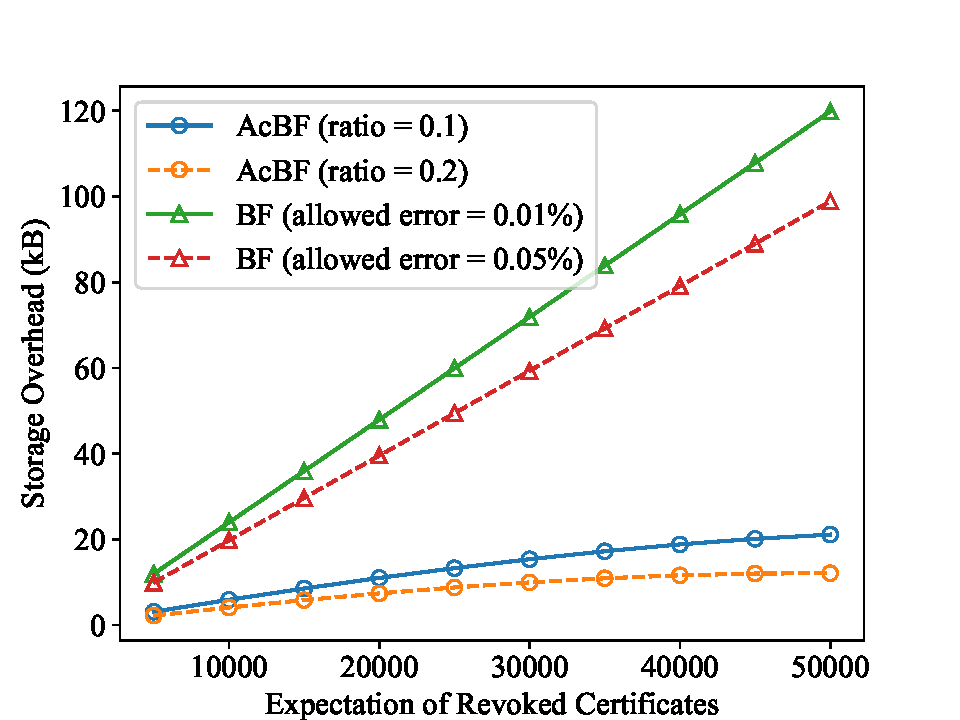
\includegraphics[width=7cm]{storage_overhead}
	\caption{Storage on Verifier Side for Revocation}\label{fig:withBF}
\end{figure}

\section{Related Works}\label{section:related}
Blockchain is a promising technology to devise reliable and decentralized certificate management. Fromknecht \textit{et al}. 
\cite{fromknechtDecentralizedPublicKey} proposed CertCoin to ensure identity retention with cryptocurrencies.  
Compared with the traditional technique like CA-based PKI \cite{pki} and PGP method \cite{pgp}, the tamper free feature brought from blockchain tackles the gap between decentralized deployment and secure certificate management, respectively. 
A totally decentralized model called SSI (self-sovereign identity) \cite{foundation_sovrin_2018} was designed by the Sovrin Foundation in 2018. In SSI, users' identities are registered in blockchain by themselves. 
%while authorities are responsible for determination the privilege of each ID with off-chain credentials. 
This idea has been realized in industrial implementations such as hyperledger indy \cite{indy} and uPort \cite{naik2020uport}, and attracted academic researches, like SmartDID \cite{smartdid}. However, the fully decentralized method does not suit practical systems, since it is complex to deal with the trust and revocation.

Another way that blockchain improves identity system is to let the blockchain manage distributed CAs and certificate revocation list (CRL). Wang \textit{et al.} \cite{CTRT} realized a transparent revocation by enabling OCSP (Online Certificate Status Protocol) on blockchain.
Chen \textit{et al}. \cite{chenCertchainPublicEfficient2018a} proposed CertChain, in which a dependability-rank based consensus organized muliptle CAs and uses double counting bloom filter (DCBF) to shorten the volume of CRL. However, Luo \textit{et al.} \cite{luoScalaCertScalabilityOrientedPKI2022a} pointed out that DCBF still occupied too much storage resource on the chain. Chameleon hash \cite{ateniese2017redactable} enables redactable blockchain such that revocation can be realized without CRL, thus many schemes were proposed, such as \cite{luoScalaCertScalabilityOrientedPKI2022a,jiaRedactableBlockchainDecentralized2022, xu2021k, jia2021process}. Note that block redaction is difficult to make everyone aware, additional mechanism shold be proposed, e.g., random freshness check \cite{luoScalaCertScalabilityOrientedPKI2022a}, RSA-based accumulator \cite{jiaRedactableBlockchainDecentralized2022} and CGBF \cite{jia2021process}. Much worse problem is that redactable blockchain does not suit lightweight node, as revoked certificate can still be ``valid'' since the block header has not varied.

Due to the similar distributed architecture, blockchain-based identity is promising to secure the future ad-hoc networks, such as IoT and IoV \cite{cui2022efficient, singh2018branch, smartdid, yu2019blockchain}. Especially, SmartDID \textit{et al.} \cite{smartdid} supports lightweight node deployment, by taking into account the latency restriction, instable links, untrust peers. Whereas, we found that the above revocation mechanisms no longer works faced with a verifier only storing block headers. It is difficult for a lightweight node to cache and update CRL in time, especially when the downlink channel is not trust. Due to similar reasons, mechanisms in \cite{luoScalaCertScalabilityOrientedPKI2022a, jiaRedactableBlockchainDecentralized2022} also failed. Some schemes leveraged MHT \cite{certledger} or accumulator \cite{yu2019blockchain} to maintain all legitimate certificates, which seems to suit lightweight node since the verifier only needs to keep up with the root node or accumulator value. 
However, they will bring in unbearable burden on certificate owners' side (which are also thin devices), as shown in Table \ref{table:compare}. 

In summary, to our best knowledge, AcBF is the first to realize revokable identity management, with extremely slight storage, computation and communication burden on both certificate owner and verifier's sides.

%Liu \textit{et al}. \cite{liuBlockchainEmpoweredCooperative2020}  proposed a decentralized and traceable collaborative authentication mechanism  by introducing the mechanism of secret sharing and dynamic proxy technology to blockchain. 

\section{Conclusion}\label{sec:conclusion}
In this paper, we proposed AcBF, which realized a blockchain-based identity system for lightweight nodes.  

\balance
\bibliographystyle{IEEEtran}
\bibliography{id}
\end{document}